\subsection{Reco changes}
New version, new channel map, pandora max iterations, explanation of the new filters, new spill time


To validate the new reconstruction, we use the Monte Carlo samples to compare the reconstructed vertex position with the true one (Figure \ref{fig:resolution_old} and Figure \ref{fig:resolution_new}).


\begin{figure}[!h]
    \centering
    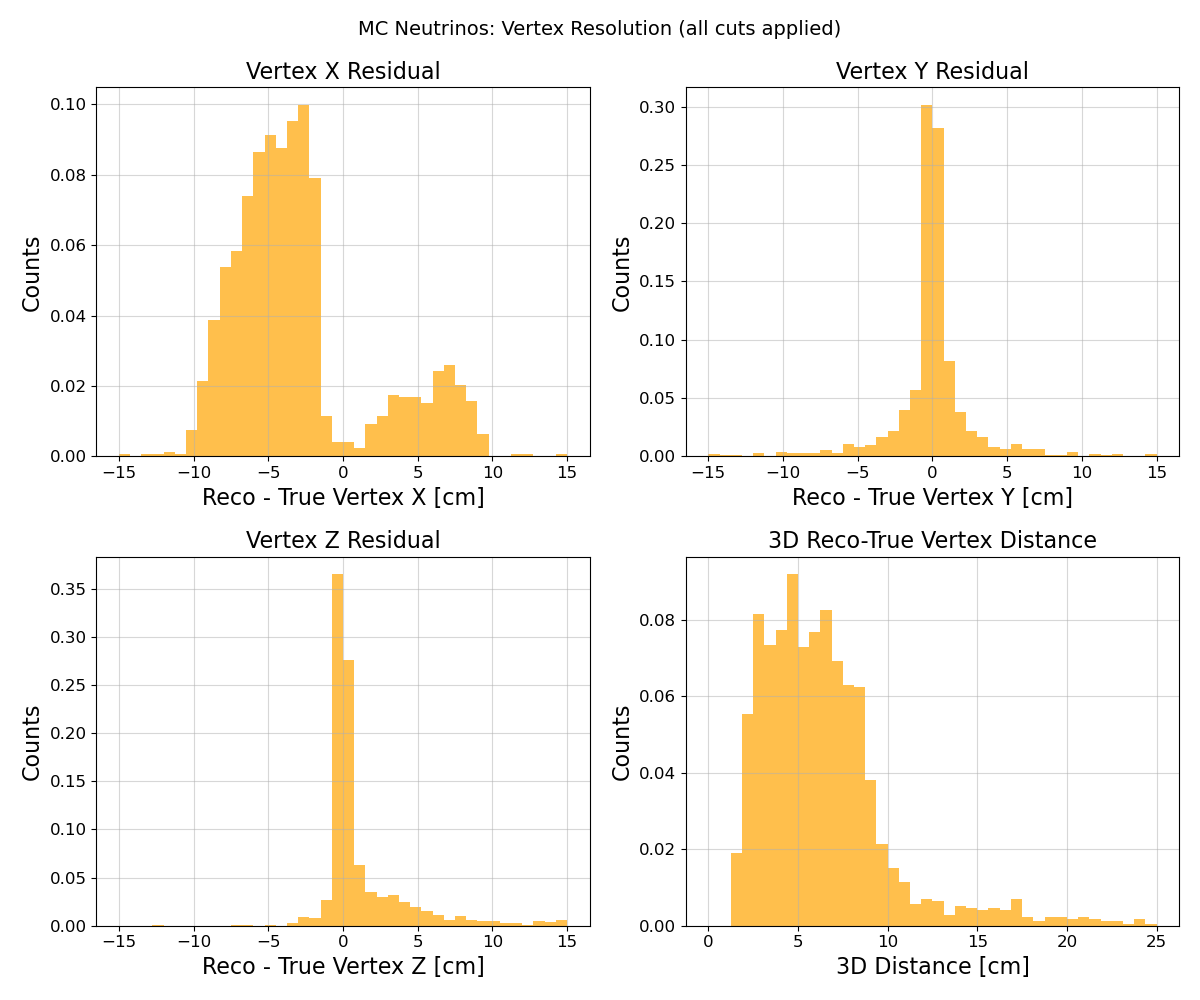
\includegraphics[width=0.87\linewidth]{sections/appendix/changes/mc_vertex_resolution_old.png}
    \caption{Old reconstruction performances, area normalized to 1. Top left: Difference between the reconstructed and true vertex X position. Top right: Difference between the reconstructed and true vertex Y position. Bottom left: Difference between the reconstructed and true vertex Z position. Bottom right: Distance in 3D between the reconstructed and true position.}
    \label{fig:resolution_old}
\end{figure}
\begin{figure}[!h]
    \centering
    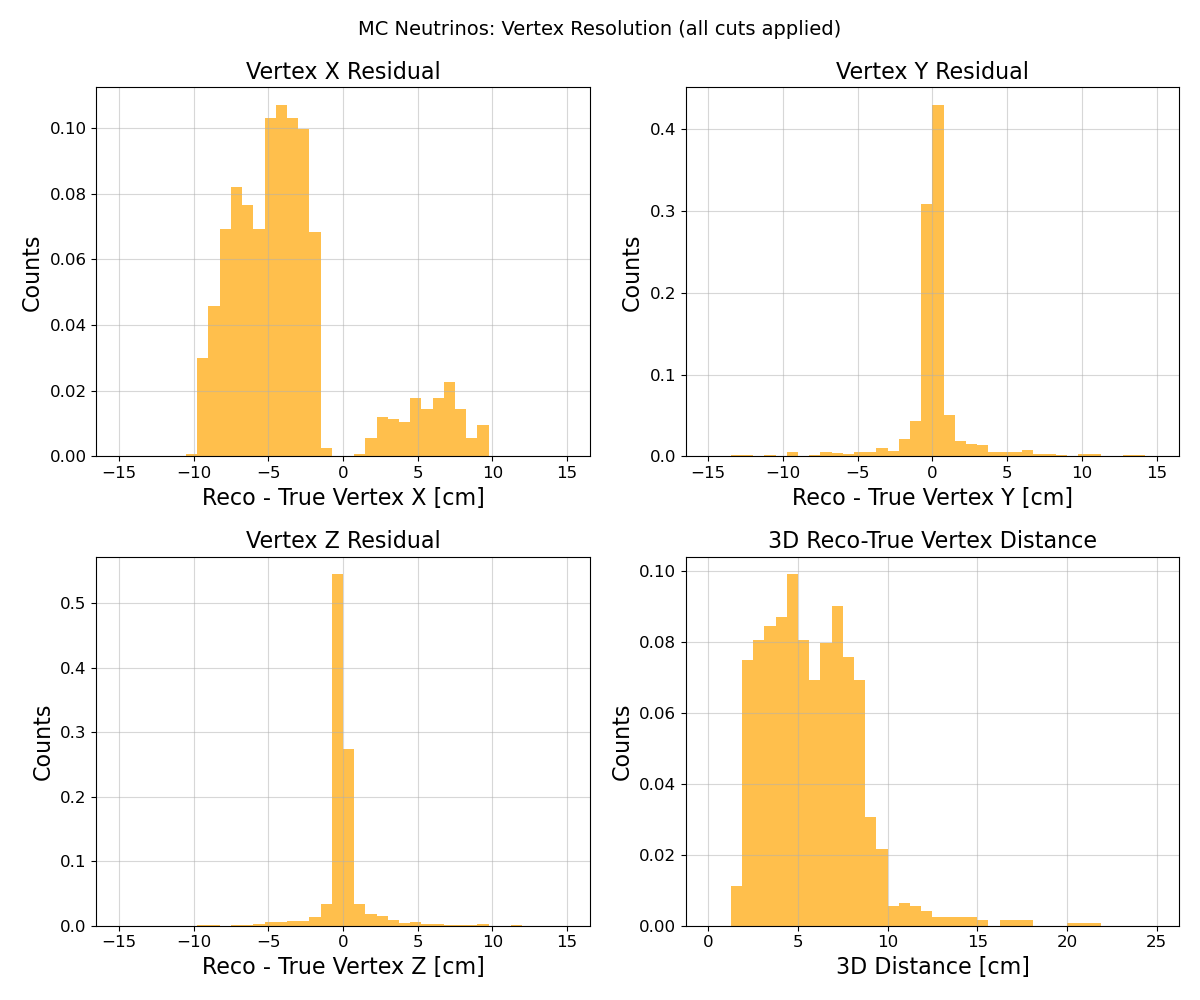
\includegraphics[width=0.87\linewidth]{sections/appendix/changes/mc_vertex_resolution_new.png}
    \caption{New reconstruction performances, area normalized to 1. Top left: Difference between the reconstructed and true vertex X position. Top right: Difference between the reconstructed and true vertex Y position. Bottom left: Difference between the reconstructed and true vertex Z position. Bottom right: Distance in 3D between the reconstructed and true position.}    
    \label{fig:resolution_new}
\end{figure}

The new reconstruction, together with the fixed channel map, improves the vertex position reconstruction significantly, mostly in the Y-Z plane. 


\subsection{Results comparison}

For reference, Table~\ref{tab:onoff_ratio_alltps_v1} reproduces the old-reconstruction selection cascade (identical to the old-reconstruction version of Table~\ref{tab:onoff_ratio_alltps} in the main Results section); see Table~\ref{tab:onoff_ratio_alltps} in the main text for the adopted new-reconstruction numbers.

\begin{table}[htbp]
\centering
\resizebox{\textwidth}{!}{%
\begin{tabular}{lccc}
\hline
Cut & Beam-off Events/h & Beam-on Events/h & Beam On/Beam Off Ratio \\
\hline
Before cuts & $1950.26 \pm 6.61$ & $2383.98 \pm 12.01$ & $1.22$ \\
Max $\cos(\theta_{\mathrm{beam}})$ & $106.34 \pm 1.54$ & $217.53 \pm 3.63$ & $2.05$ \\
Tail Length Density & $23.09 \pm 0.72$ & $28.96 \pm 1.32$ & $1.25$ \\
Cut on $C_{140-150}$ & $6.65 \pm 0.39$ & $9.92 \pm 0.77$ & $1.49$ \\
ROI Z close to vertex & $1.79 \pm 0.20$ & $3.87 \pm 0.48$ & $2.16$ \\
N daughter particles & $0.81 \pm 0.13$ & $2.84 \pm 0.41$ & $3.53$ \\
Vertex fiducial volume & $0.65 \pm 0.12$ & $2.48 \pm 0.39$ & $3.82$ \\
Cut on $C_{40-50}$ & $0.56 \pm 0.11$ & $2.36 \pm 0.38$ & $4.21$ \\
ROI Z size & $0.49 \pm 0.10$ & $2.12 \pm 0.36$ & $4.30$ \\
Cut on $C_{0-10}$ & $0.45 \pm 0.10$ & $1.87 \pm 0.34$ & $4.19$ \\
\hline
\end{tabular}
}
\caption{Old reconstruction: beam-on and beam-off events per hour with the corresponding ratio for various selection cuts, considering all the available time with the spill on. This is the old-reconstruction cascade that Table~\ref{tab:onoff_ratio_alltps} in the main text has now replaced.}
\label{tab:onoff_ratio_alltps_v1}
\end{table}

Between the old and new reconstruction, the number of events that pass all selection cuts has increased from 31 to 60, using the exact same selection criteria. 





\subsection{Old reconstruction: Results headline}

The following reproduces the old-reconstruction versions of the headline Results-section content that has now been replaced in the main text by the new-reconstruction reprocessing.

\begin{table}[htbp]
    \centering
    \begin{tabular}{|c|c|c|c|}
        \hline
         & Number of events & Time (hours) & Hourly rate\\
        \hline
        Beam-on & 31 & 16.53 & 1.88 \\
        \hline
        Beam-off & 20 & 44.688 & 0.45\\
        \hline
    \end{tabular}
    \caption{Old reconstruction: observed number of events that pass all selection cuts, and total live time available. Superseded by Table~\ref{tab:post_cut_numbers_all_tps} in the main text ($\text{N}_{\text{ON}}$ updated to 60, giving $10.23\sigma$ in place of this old-reconstruction count's $6.35\sigma$).}
    \label{tab:post_cut_numbers_all_tps_v1}
\end{table}

Using the old-reconstruction event counts above, the simple Poisson significance formula (Eq.~\ref{eq:basic_formula}) gave $6.35\sigma$, with MCMC most-probable rates $\text{R}_{\text{neutrino}}=1.429$ and $\text{R}_{\text{background}}=0.455$ (Figure~\ref{fig:mcmc_approach_all_v1}).

\begin{figure}[h]
    \centering
    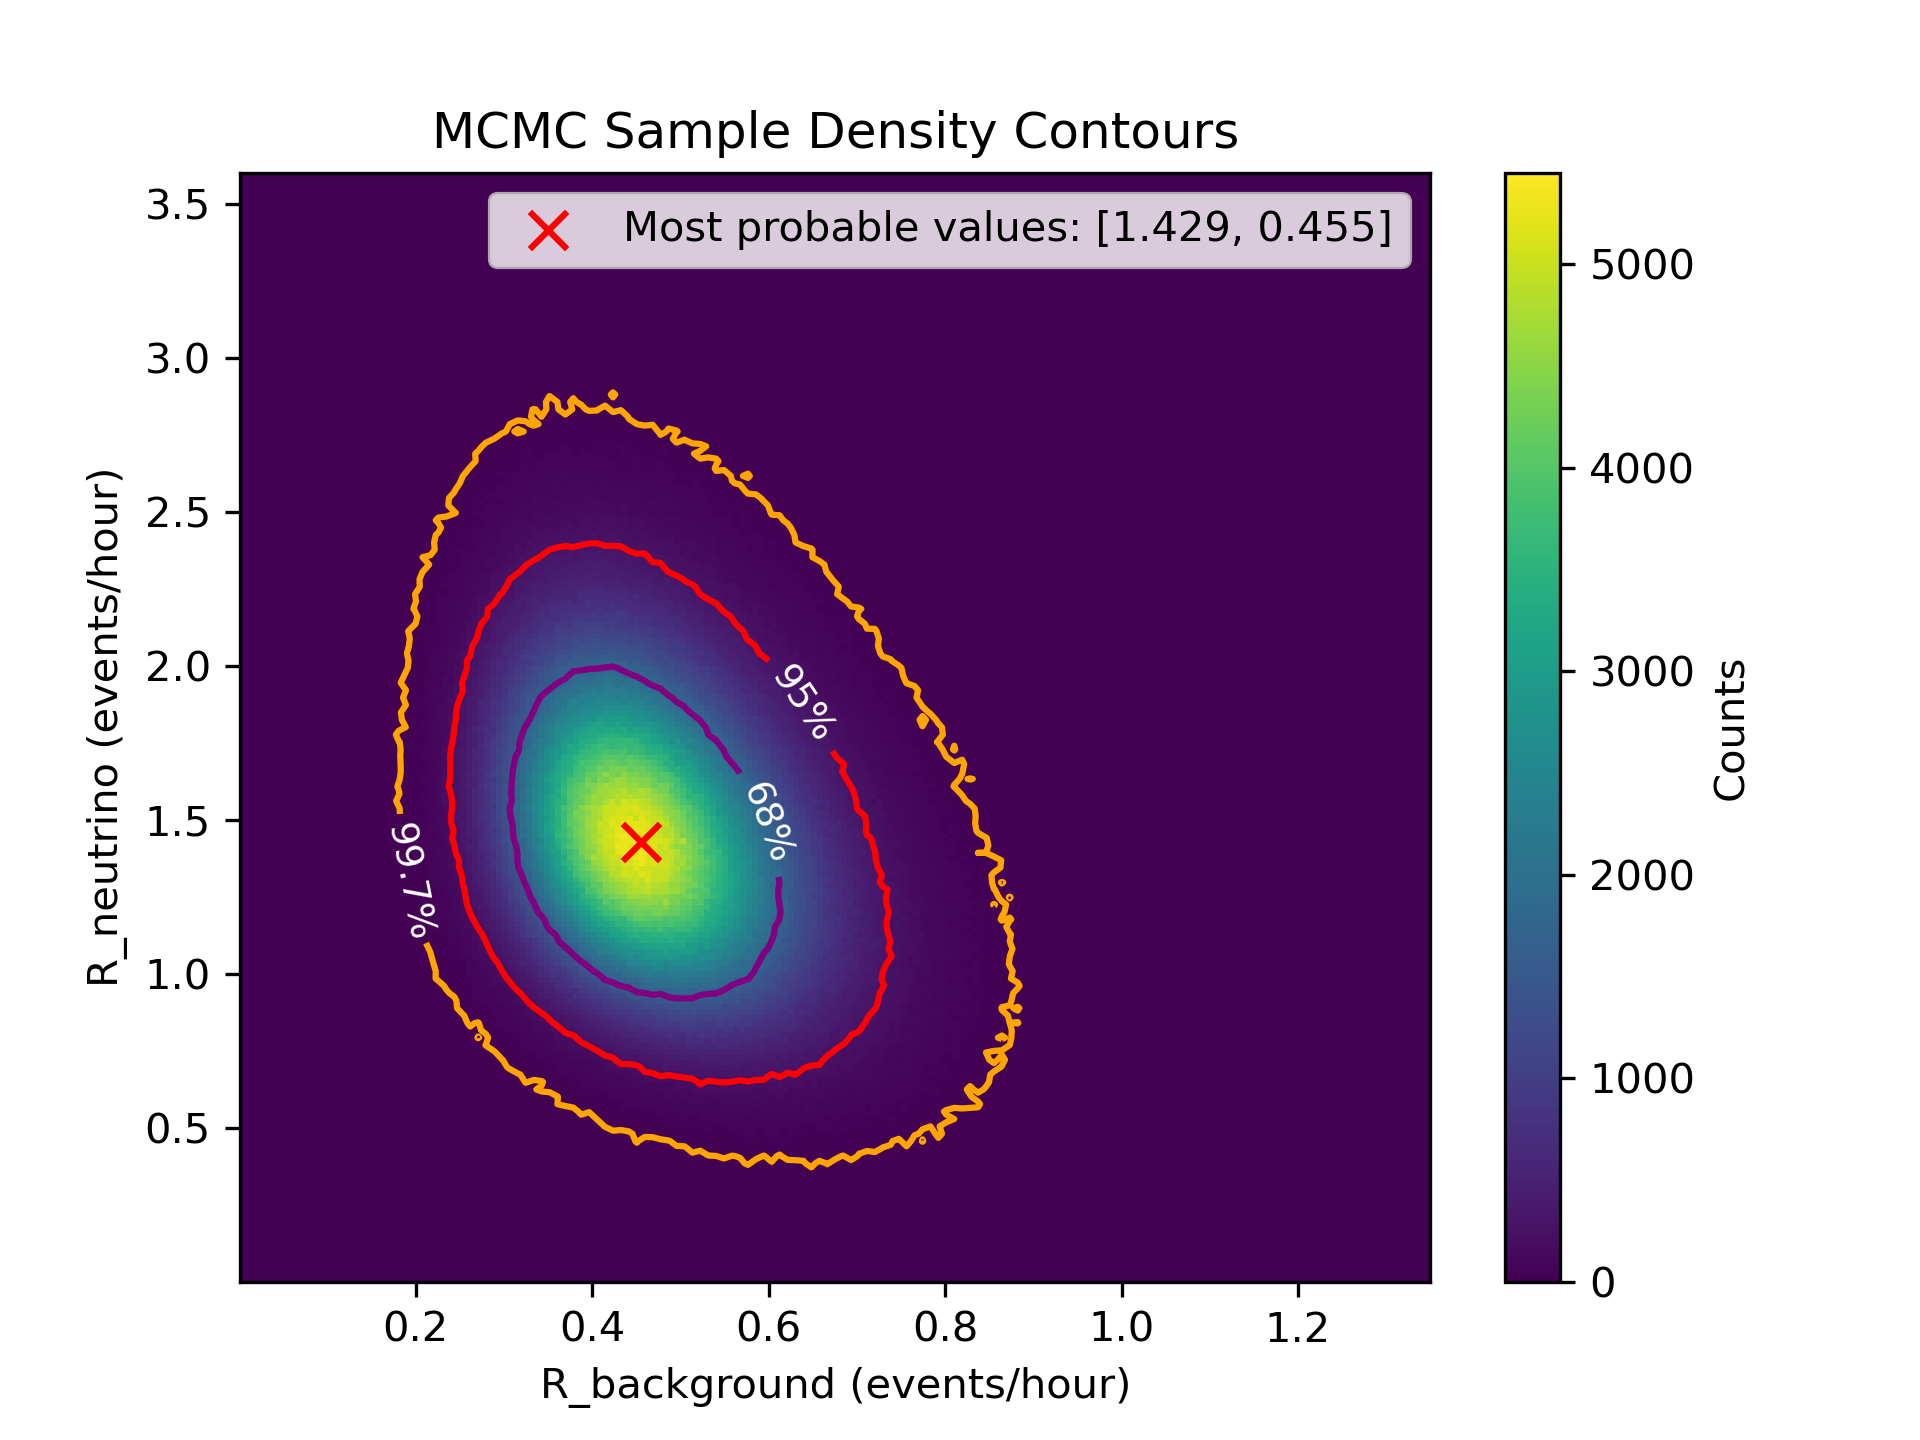
\includegraphics[width=0.69\linewidth]{sections/appendix/legacy_v1_plots/results_significance/mcmc_contours_all.png}
    \caption{Old reconstruction: histogram of the sampled $\log(\mathcal{L}_{\text{Poisson}})$ using the Monte Carlo method. Superseded by Figure~\ref{fig:mcmc_approach_all} in the main text.}
    \label{fig:mcmc_approach_all_v1}
\end{figure}

\begin{figure}[h]
    \centering
    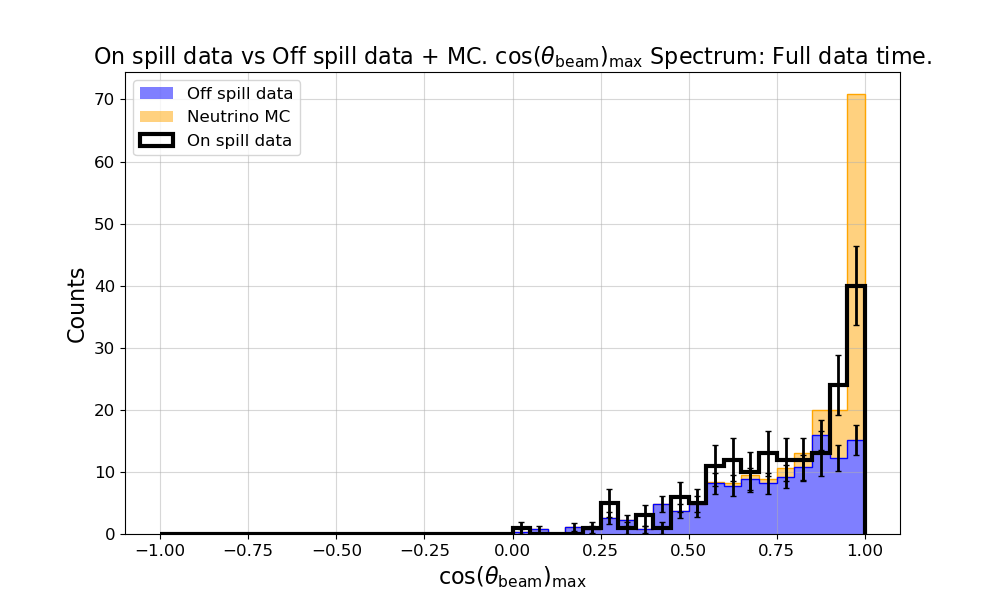
\includegraphics[width=0.69\linewidth]{sections/plots/version_1/beam_on_vs_off/output_test_full_time_all_tps/sig_bkg_mc_max_directionZ_directionZ2_spectrum_full_sig_time.png}
    \caption{Old reconstruction: distribution of $\cos(\theta_{\mathrm{beam}})_\text{max}$ comparing beam-on data with the stacked distributions of beam-off and Monte Carlo neutrinos. Superseded by Figure~\ref{fig:beam_on_maxZ_all_tps} in the main text.}
    \label{fig:beam_on_maxZ_all_tps_v1}
\end{figure}

\begin{figure}[h]
    \centering
    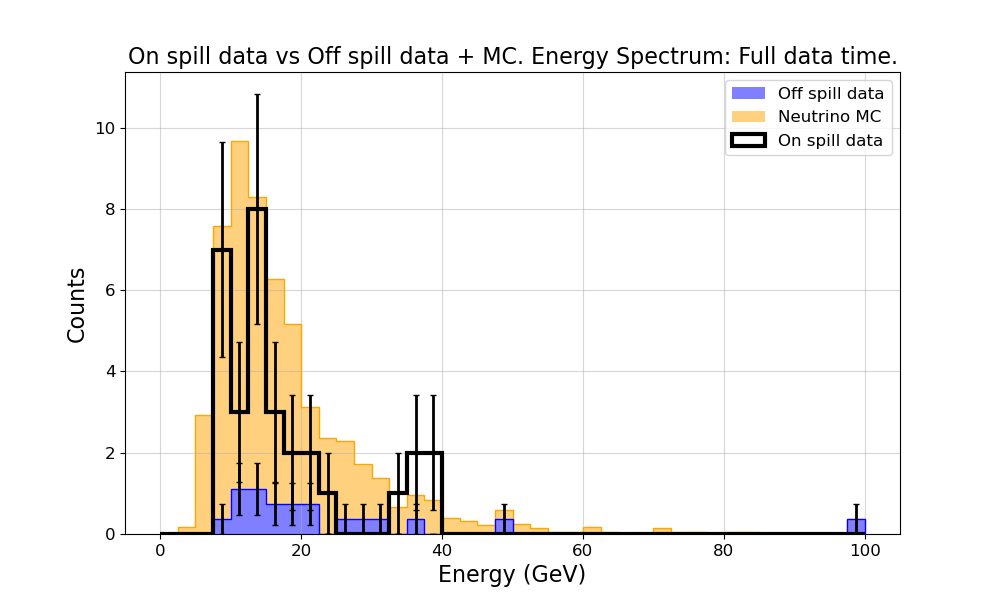
\includegraphics[width=0.69\linewidth]{sections/plots/version_1/beam_on_vs_off/output_test_full_time_all_tps/sig_bkg_mc_energy_spectrum_full_sig_time.png}
    \caption{Old reconstruction: deposited energy spectrum comparing beam-on data with the stacked distributions of beam-off and Monte Carlo neutrinos. Superseded by Figure~\ref{fig:beam_on_energy_all_tps} in the main text.}
    \label{fig:beam_on_energy_all_tps_v1}
\end{figure}

\begin{figure}[h]
    \centering
    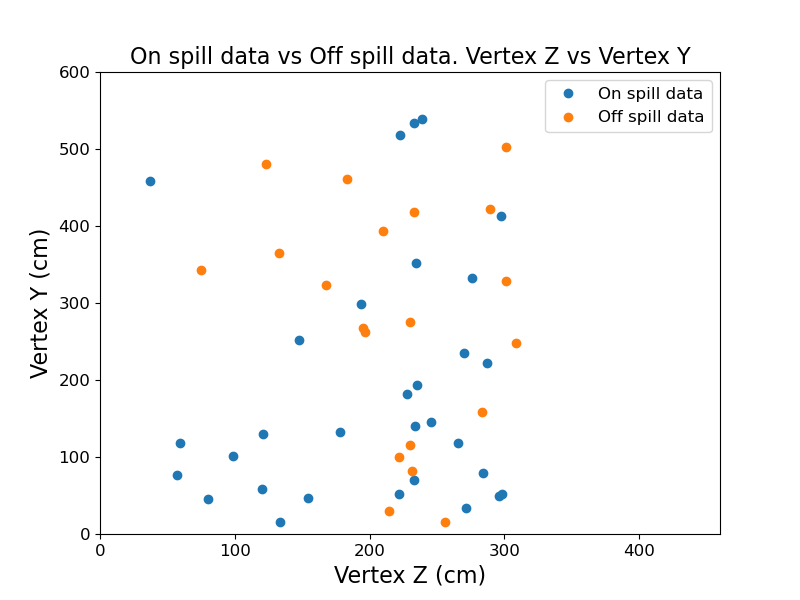
\includegraphics[width=0.69\linewidth]{sections/plots/version_1/beam_on_vs_off/output_test_full_time_all_tps/sig_bkg_vertexZ_vs_vertexY_scatter.png}
    \caption{Old reconstruction: vertex position in the ZY plane for the spill-on and spill-off events that pass all selections, considering all the available spill on time. Superseded by Figure~\ref{fig:vertex_position_yz_all_tps} in the main text.}
    \label{fig:vertex_position_yz_all_tps_v1}
\end{figure}

\clearpage
\subsection{Old reconstruction: Analysis headline}

The following reproduces the old-reconstruction versions of the Analysis-section selection-cut headline content that has now been replaced in the main text by the new-reconstruction reprocessing.

\begin{table}[htbp]
\centering
\resizebox{\textwidth}{!}{%
\begin{tabular}{lccc}
\hline
Cut & Bkg Events & Signal Events & Sig/Bkg Ratio \\
\hline
Before cuts & 1950.26 $\pm$ 6.61  & 20.91 & 0.01 \\
Max $\cos(\theta_{\mathrm{beam}})$ & 106.34 $\pm$ 1.54 & 10.12 & 0.10 \\
Tail Length Density & 23.09 $\pm$ 0.72 & 6.60 & 0.29 \\
Cut on $C_{140-150}$ & 6.65 $\pm$ 0.39 & 4.57 & 0.69 \\
ROI Z close to vertex & 1.79 $\pm$ 0.20 & 3.88 & 2.17 \\
N daughter particles & 0.81 $\pm$ 0.13 & 3.44 & 4.26 \\
Vertex fiducial volume & 0.65 $\pm$ 0.12 & 3.37 & 5.20 \\
Cut on $C_{40-50}$ & 0.56 $\pm$ 0.11 & 3.13 & 5.60 \\
ROI Z size & 0.49 $\pm$ 0.10 & 3.11 & 6.32 \\
Cut on $C_{0-10}$ & 0.45 $\pm$ 0.10 & 2.99 & 6.69 \\
\hline
Surviving events & 0.02\% & 14.2\% & \\
\hline
\end{tabular}
}
\caption{Old reconstruction: expected number of events during all steps of the selection, weighted to one hour of beam-on data. Superseded by Table~\ref{tab:filter_evolution} in the main text.}
\label{tab:filter_evolution_v1}
\end{table}

\begin{figure}[!h]
    \centering
    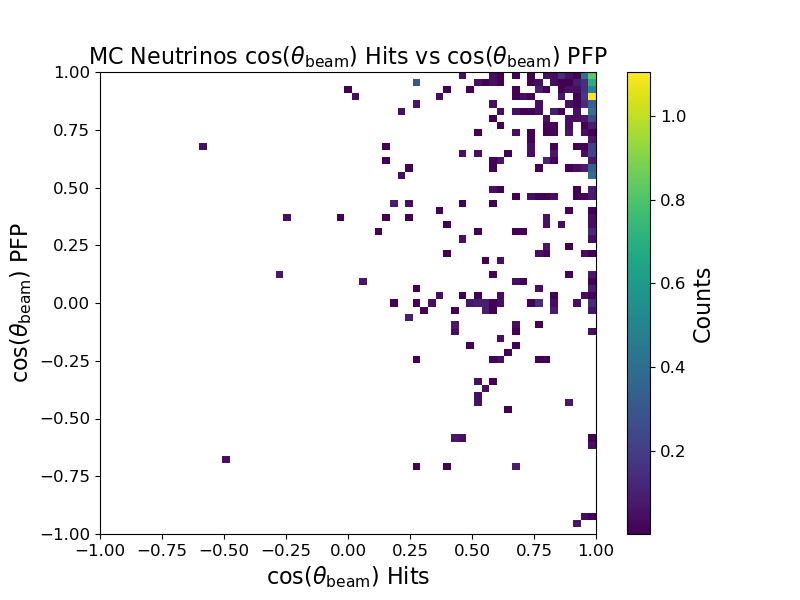
\includegraphics[width=0.59\linewidth]{sections/appendix/legacy_v1_plots/analysis_selection/sig_directionZ_vs_directionZ2.png}
    \caption{Old reconstruction: 2D histogram showing the $\cos(\theta_{\mathrm{beam}})$ computed with two different reconstruction methods. Superseded by Figure~\ref{fig:z1_vs_z2} in the main text.}
    \label{fig:z1_vs_z2_v1}
\end{figure}
\begin{figure}[!h]
    \centering
    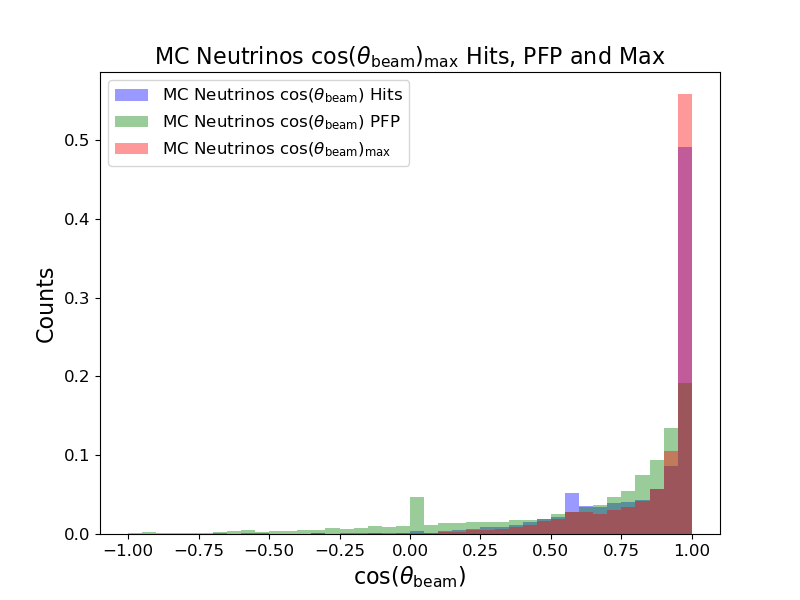
\includegraphics[width=0.49\linewidth]{sections/appendix/legacy_v1_plots/analysis_selection/sig_direction_histograms.png}
    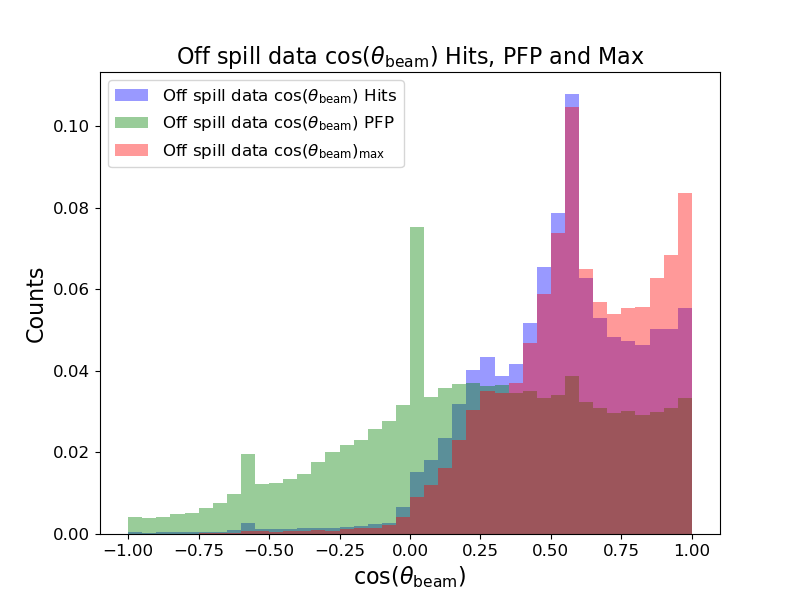
\includegraphics[width=0.49\linewidth]{sections/appendix/legacy_v1_plots/analysis_selection/bkg_direction_histograms.png}
    \caption{Old reconstruction: 1D histograms showing the $\cos(\theta_{\mathrm{beam}})$ computed with two different reconstruction methods and the maximum value between the two for the Monte Carlo neutrinos (left) and the spill-off data (right). Superseded by Figure~\ref{fig:z1_vs_z2_1d} in the main text.}
    \label{fig:z1_vs_z2_1d_v1}
\end{figure}

\clearpage
\subsection{Old reconstruction: High/Low TP validation}

The following reproduces the old-reconstruction versions of the "High TP vs Low TP validation" content that has now been replaced in the main text by the new-reconstruction reprocessing, including the significance result (now $6.44\sigma$, see Section~\ref{chap:significance_method} and the "High TP vs Low TP validation" subsection of the Results).

\begin{table}[htbp]
\centering
\resizebox{\textwidth}{!}{%
\begin{tabular}{lccc}
\hline
Cut & Beam-off Events/h & Beam-on Events/h (High TP) & Beam-on Events/h (Low TP) \\
\hline
Before cuts & $1950.26 \pm 6.61$ & $2911.81 \pm 18.99$ & $1880.33 \pm 14.90$ \\
Max $\cos(\theta_{\mathrm{beam}})$ & $106.34 \pm 1.54$ & $330.11 \pm 6.39$ & $110.11 \pm 3.61$ \\
Tail Length Density & $23.09 \pm 0.72$ & $35.91 \pm 2.11$ & $22.33 \pm 1.62$ \\
Cut on $C_{140-150}$ & $6.65 \pm 0.39$ & $11.64 \pm 1.20$ & $8.27 \pm 0.99$ \\
ROI Z close to vertex & $1.79 \pm 0.20$ & $4.09 \pm 0.71$ & $3.66 \pm 0.66$ \\
N daughter particles & $0.81 \pm 0.13$ & $2.97 \pm 0.61$ & $2.72 \pm 0.57$ \\
Vertex fiducial volume & $0.65 \pm 0.12$ & $2.60 \pm 0.57$ & $2.36 \pm 0.53$ \\
Cut on $C_{40-50}$ & $0.56 \pm 0.11$ & $2.60 \pm 0.57$ & $2.13 \pm 0.50$ \\
ROI Z size 10 cm & $0.49 \pm 0.10$ & $2.48 \pm 0.55$ & $1.77 \pm 0.46$ \\
Cut on $C_{0-10}$ & $0.45 \pm 0.10$ & $2.10 \pm 0.51$ & $1.65 \pm 0.44$ \\
\hline
\end{tabular}
}
\caption{Old reconstruction: beam-on and beam-off events per hour for various selection cuts, comparing high TP and low TP rate periods. Superseded by Table~\ref{tab:onoff_ratio_high_low_tps} in the main text.}
\label{tab:onoff_ratio_high_low_tps_v1}
\end{table}

\begin{table}[htbp]
    \centering
    \begin{tabular}{|c|c|c|c|}
        \hline
         & Number of events & Time (hours) & Hourly rate\\
        \hline
        Beam-on & 14 & 8.463 & 1.65 \\
        \hline
        Beam-off & 20 & 44.688 & 0.45\\
        \hline
    \end{tabular}
    \caption{Old reconstruction: observed number of events that pass all selection cuts, considering the full beam off data and only the beam on time with a low TP rate. Superseded by Table~\ref{tab:post_cut_numbers_low_tps} in the main text ($\text{N}_{\text{ON}}$ updated to 27, giving $6.44\sigma$ in place of this old-reconstruction count's $3.85\sigma$).}
    \label{tab:post_cut_numbers_low_tps_v1}
\end{table}

\begin{figure}[h]
    \centering
    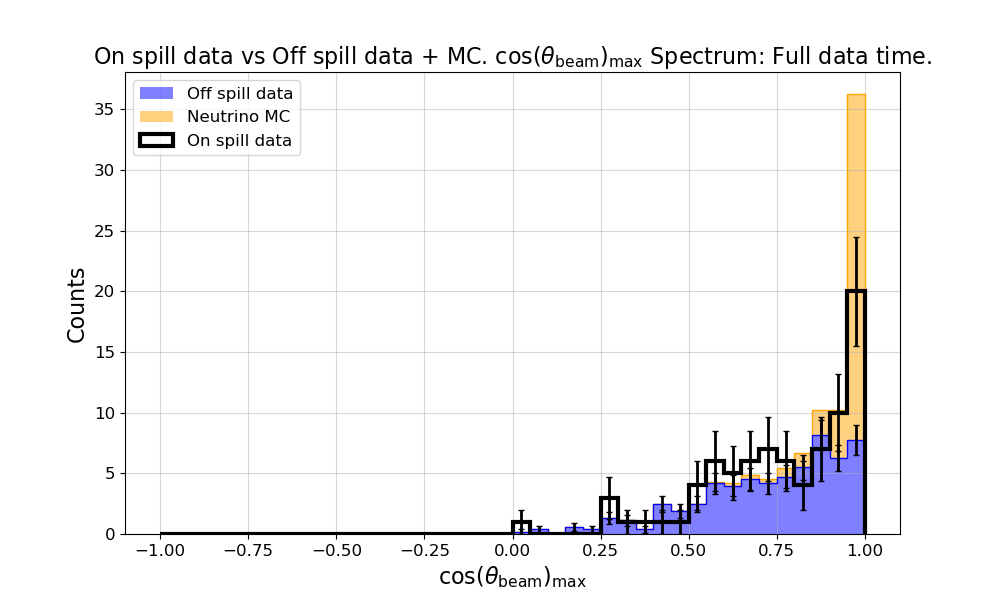
\includegraphics[width=0.49\linewidth]{sections/plots/version_1/beam_on_vs_off/output_test_full_time/sig_bkg_mc_max_directionZ_directionZ2_spectrum_full_sig_time.png}
    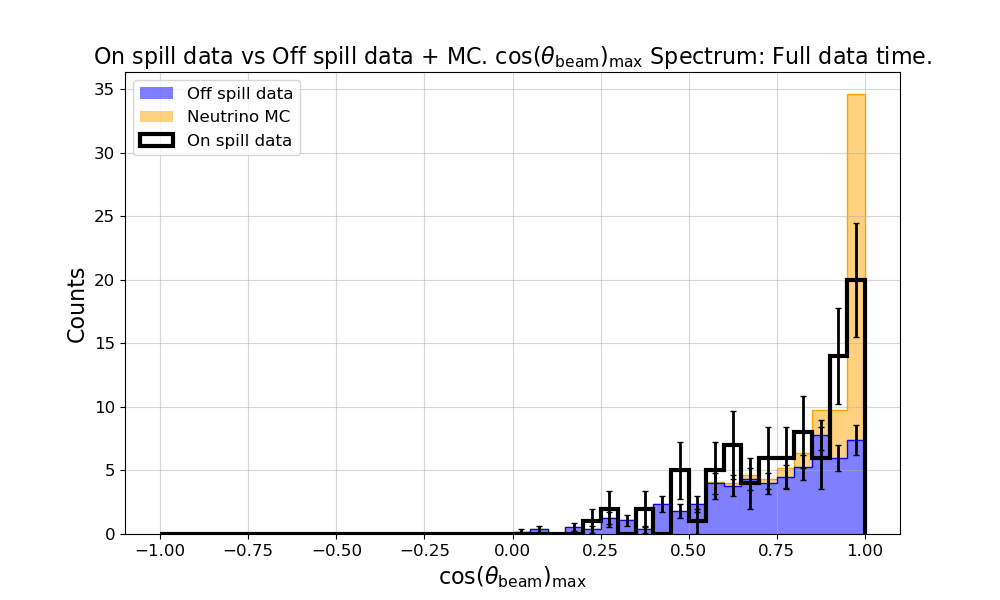
\includegraphics[width=0.49\linewidth]{sections/plots/version_1/beam_on_vs_off/full_time_high_tps/sig_bkg_mc_max_directionZ_directionZ2_spectrum_full_sig_time.png}
    \caption{Old reconstruction: distribution of $\cos(\theta_{\mathrm{beam}})_\text{max}$ with the low TP rate (left) and the high TP rate (right). Superseded by Figure~\ref{fig:max_cos_theta_high_low} in the main text.}
    \label{fig:max_cos_theta_high_low_v1}
\end{figure}

\begin{figure}[h]
    \centering
    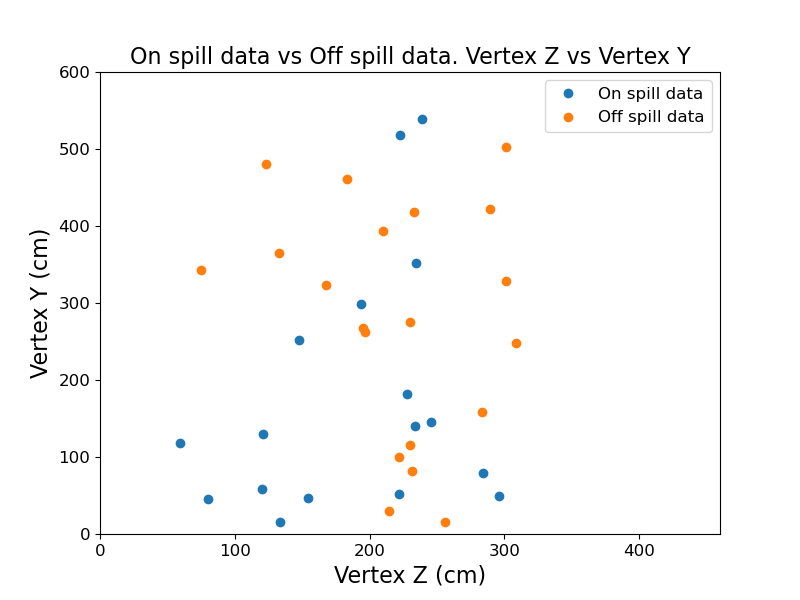
\includegraphics[width=0.69\linewidth]{sections/plots/version_1/beam_on_vs_off/full_time_high_tps/sig_bkg_vertexZ_vs_vertexY_scatter.png}
    \caption{Old reconstruction: vertex position in the ZY plane for the spill-on and spill-off events that pass all selections, considering the time period with a visible increase in the TP rate corresponding to the beam spill. Superseded by Figure~\ref{fig:vertex_position_yz_high_tps} in the main text.}
    \label{fig:vertex_position_yz_high_tps_v1}
\end{figure}

\begin{figure}[h]
    \centering
    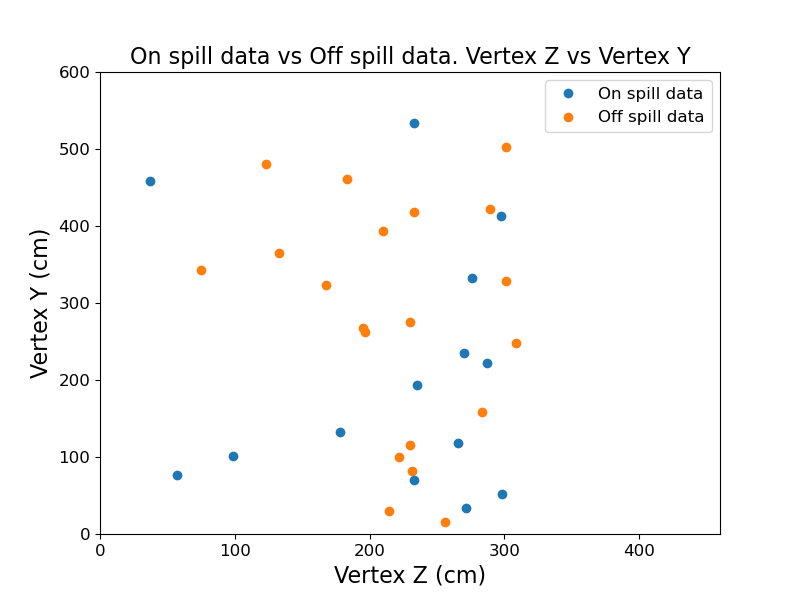
\includegraphics[width=0.69\linewidth]{sections/appendix/legacy_v1_plots/results_significance/generic_vertexZ_vs_vertexY_scatter_v1.png}
    \caption{Old reconstruction: vertex position in the ZY plane for the spill-on and spill-off events that pass all selections (generic/combined plot used in place of a dedicated low-TP scatter prior to the new reconstruction). Superseded by Figure~\ref{fig:vertex_position_yz} in the main text, which now shows a genuine low-TP-only scatter.}
    \label{fig:vertex_position_yz_v1}
\end{figure}

\begin{figure}[h]
    \centering
    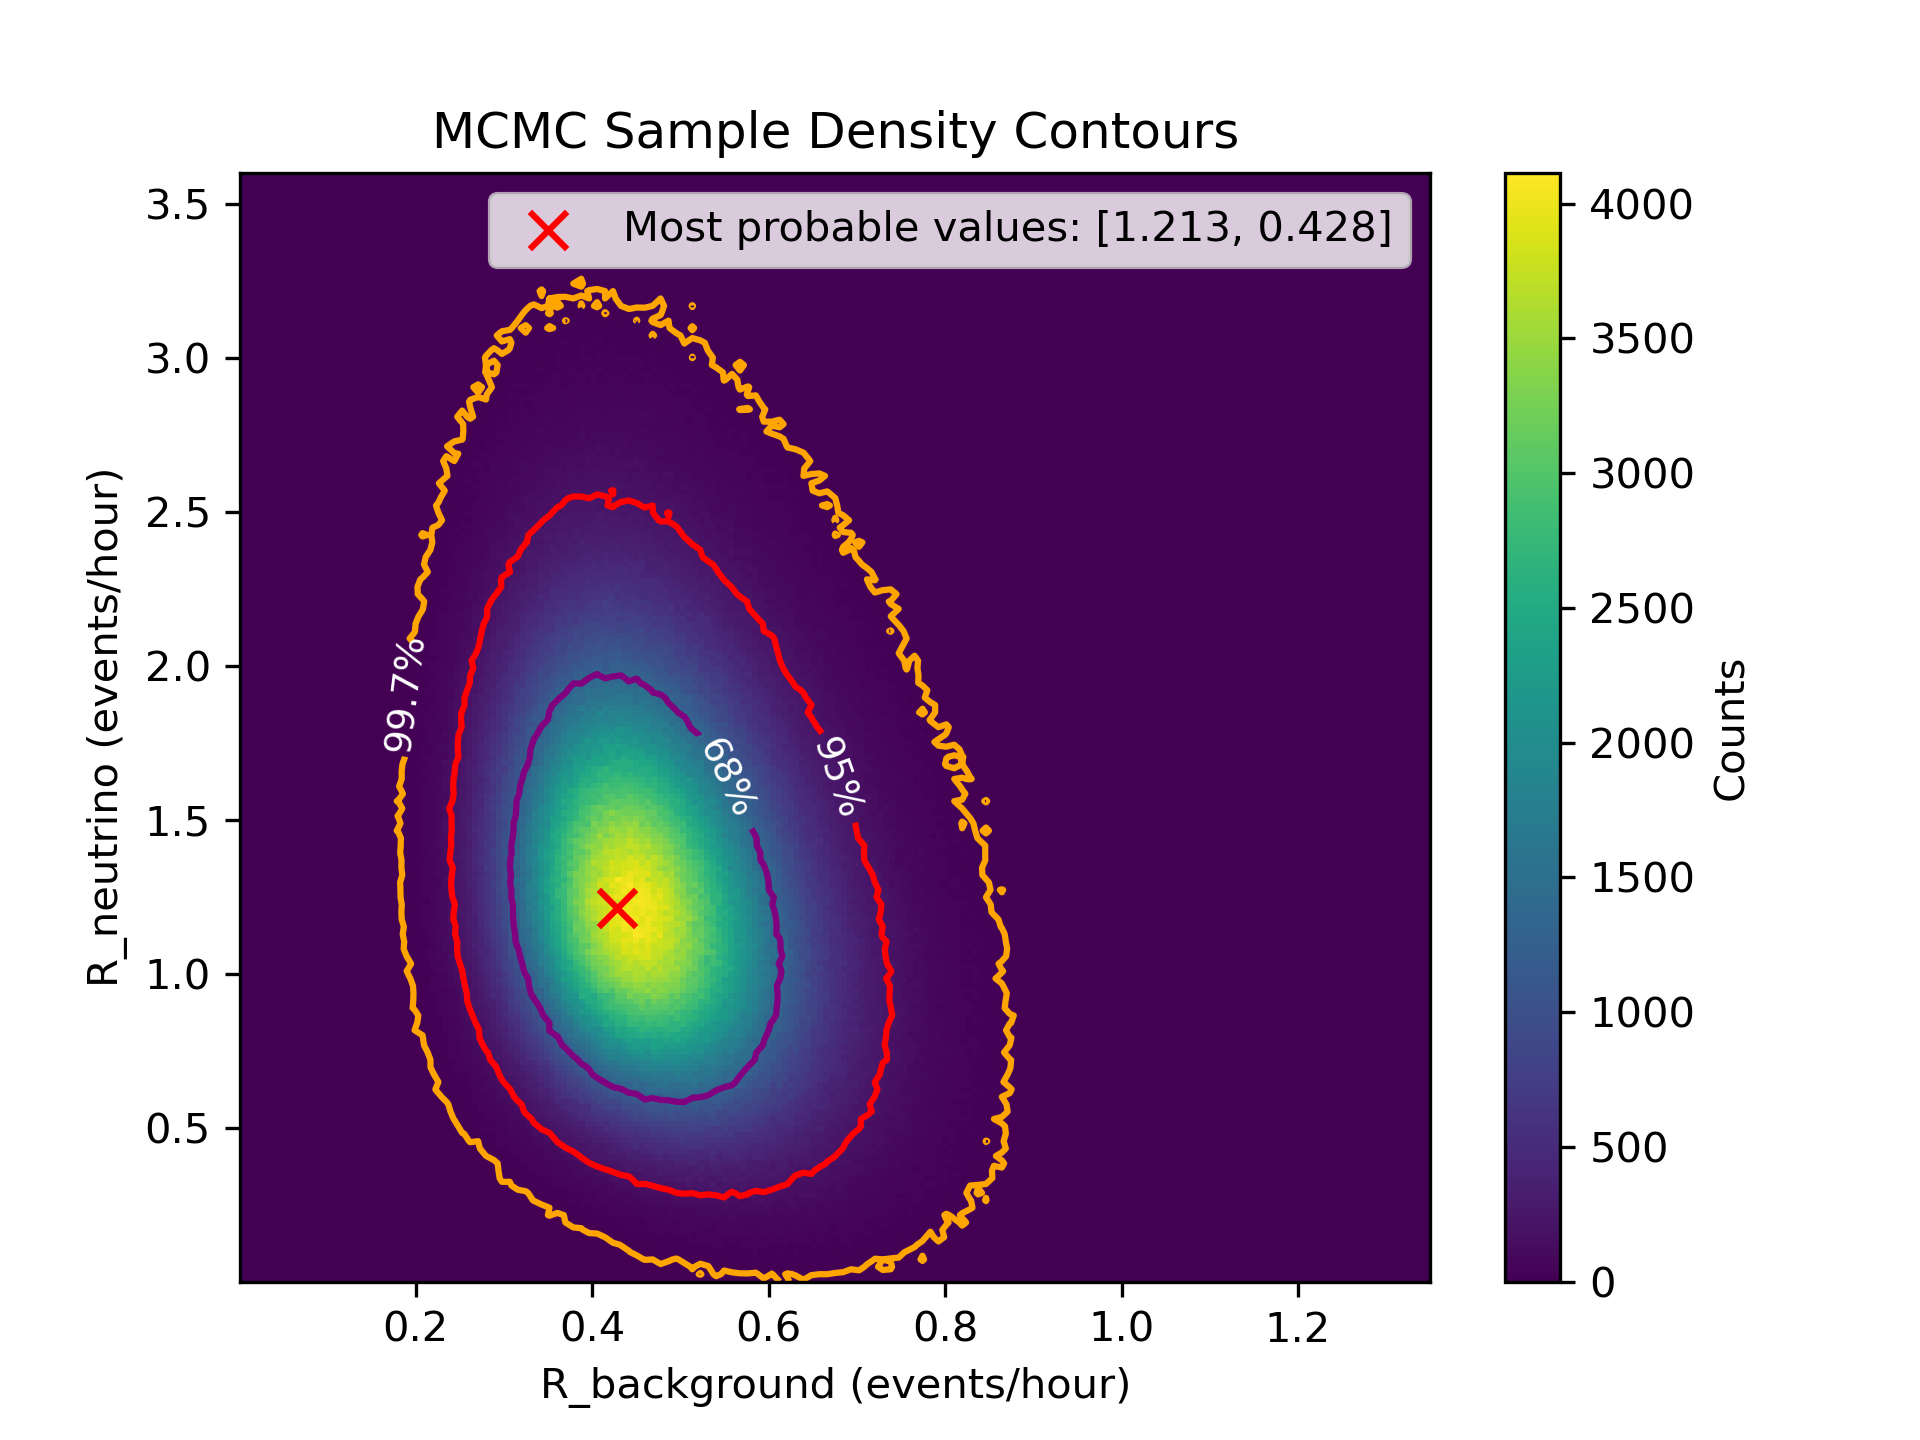
\includegraphics[width=0.69\linewidth]{sections/appendix/legacy_v1_plots/results_significance/mcmc_contours_low.png}
    \caption{Old reconstruction: histogram of the sampled $\log(\mathcal{L}_{\text{Poisson}})$ using the Monte Carlo method, low-TP-only sample ($\text{N}_{\text{ON}}=14$, giving $3.85\sigma$). Superseded by Figure~\ref{fig:mcmc_approach} in the main text.}
    \label{fig:mcmc_approach_low_v1}
\end{figure}

